
%(BEGIN_QUESTION)
% Copyright 2011, Tony R. Kuphaldt, released under the Creative Commons Attribution License (v 1.0)
% This means you may do almost anything with this work of mine, so long as you give me proper credit

Suppose two radio antennas are located on 12-foot towers, with free and open space in between.  If their operating frequency is 900 MHz, calculate the distance between these towers where the first Fresnel zone contacts the ground in between.  Is this tower-to-tower distance a {\it minimum} or a {\it maximum} value for practical radio operation?

$$\includegraphics[width=15.5cm]{i00449x01.eps}$$

\vskip 20pt \vbox{\hrule \hbox{\strut \vrule{} {\bf Suggestions for Socratic discussion} \vrule} \hrule}

\begin{itemize}
\item{} Identify at least one practical factor which would change the distance value allowable between the two antennas.  In other words, what could change in the system to permit a different distance between antennas?
\end{itemize}

\underbar{file i00449}
%(END_QUESTION)





%(BEGIN_ANSWER)

The formula for calculating the radius of the Fresnel zone is:

$$r = \sqrt{{n \lambda d_1 d_2} \over D}$$

Since we are interested in finding the radius of the Fresnel zone at its mid-point where $d_1 = d_2 = {D \over 2}$, we may make this substitution within the formula: 

$$r = \sqrt{{n \lambda \left({D \over 2}\right)^2} \over D}$$

Simplifying:

$$r = \sqrt{n \lambda {D^2 \over 4} \over D}$$

$$r = \sqrt{n \lambda D^2 \over 4D}$$

$$r = \sqrt{n \lambda D \over 4}$$

Solving for wavelength ($\lambda$) at the operating frequency of 900 MHz and then solving for the distance given a first Fresnel zone radius of 12 feet (3.6576 meters):

$$\lambda = {v \over f} = {2.9979 \times 10^{8} \hbox{ m/s} \over 900 \times 10^6 \hbox{ Hz}} = 0.3331 \hbox{ m}$$

$$r = \sqrt{\lambda D \over 4}$$

$$r^2 = {\lambda D \over 4}$$

$$4r^2 = \lambda D$$

$$D = {4r^2 \over \lambda} = {(4) (3.6576 \hbox{ m})^2 \over 0.3331 \hbox{ m}} = 160.65 \hbox{ m}$$

$$\left(160.65 \hbox{ m} \over 1 \right) \left(100 \hbox{ cm} \over 1 \hbox{ m} \right) \left(1 \hbox{ in} \over 2.54 \hbox{ cm} \right) \left(1 \hbox{ ft} \over 12 \hbox{ in} \right) = 527.06 \hbox{ ft}$$

This distance figure is a {\it maximum}, not a minimum.  Exceeding 160.65 meters will result in the first Fresnel zone contacting the ground mid-way between the antennas.

%(END_ANSWER)





%(BEGIN_NOTES)







\vfil \eject

\noindent
{\bf Summary Quiz:}

As the frequency of a radio signal is increased:

\begin{itemize}
\item{} Path loss increases and the Fresnel zone becomes narrower
\vskip 5pt 
\item{} Path loss increases and the Fresnel zone becomes wider
\vskip 5pt 
\item{} Path loss remains unchanged and the Fresnel zone becomes narrower
\vskip 5pt 
\item{} Path loss decreases and the Fresnel zone becomes narrower
\vskip 5pt 
\item{} Path loss decreases and the Fresnel zone becomes wider
\vskip 5pt 
\item{} Path loss increases and the Fresnel zone remains unchanged
\end{itemize}


%INDEX% Electronics review, Fresnel zones for radio links

%(END_NOTES)


